% Paper #1 - English manuscript (P1.10 rewrite, Khung A, 2026-10-08).
% Build: tectonic main_en.tex   (XeTeX + BibTeX, see README.md)
% Target journal: Structural and Multidisciplinary Optimization (decision C4).
% All numbers: pipeline without periodic-edge enforcement (decision C5),
% from outputs/phase5/plan_v3/p1_9_nofp_summary.json unless noted in a
% comment next to the number. Previous draft: archive/main_en_2026-09-30.tex.
\documentclass[a4paper,11pt]{article}

\usepackage{fontspec}
\setmainfont{texgyretermes}[Extension=.otf,UprightFont=*-regular,BoldFont=*-bold,ItalicFont=*-italic,BoldItalicFont=*-bolditalic]
\usepackage[english]{babel}
\setlength{\emergencystretch}{2em}
\usepackage{amsmath,amssymb}
\usepackage{graphicx}
\usepackage{booktabs}
\usepackage{multirow}
\usepackage[margin=2.4cm]{geometry}
\usepackage[numbers,sort&compress]{natbib}
\usepackage{caption}
\captionsetup{font=small,labelfont=bf}
\usepackage{tikz}
\usetikzlibrary{arrows.meta,positioning,fit}
\usepackage[colorlinks=true,linkcolor=blue!50!black,citecolor=blue!50!black,urlcolor=blue!50!black]{hyperref}

\newcommand{\nuot}{\nu_{12}}
\newcommand{\nuto}{\nu_{21}}
\newcommand{\RR}{R^2}

\title{Optimizing What Is Verified: Binarization-Aware Latent Refinement for
Generative Inverse Design of Auxetic Metamaterials}
\author{Trịnh Bình Minh\thanks{[Affiliation and corresponding-author details to be inserted.]}}
\date{Draft, \today}

\begin{document}
\maketitle

% Abstract: SMO limit 250 words.
\begin{abstract}
Gradient-based design of metamaterial unit cells, whether by topology
optimization or by searching the latent space of a generative model, is
judged by finite-element (FE) analysis of a binarized design, yet it usually
optimizes a continuous density field. We show that this mismatch is
systematically exploited. Refining the latent code of a conditional
variational autoencoder (cVAE) against exact homogenization sensitivities
drives the objective to $\sim\!10^{-10}$ while the verified error stays six
orders of magnitude larger, and density-based topology optimization with
Heaviside continuation to $\beta=64$ shows the same gap. Placing the
verification operators inside the refinement objective raises the
FE-verified $\RR$ of the Poisson ratio $\nuot$ of two-dimensional auxetic
cells from 0.874 to 0.999 for single samples (0.831 to 0.989 on a second,
disjoint target set) and lowers the error after best-of-30 selection by
59--68\% on three disjoint sets. Against topology optimization from scratch
with four starting topologies, the generative pipeline reaches the same
accuracy with about eight times fewer FE solves and, for targets of moderate
anisotropy, a 35--41\% lower joint error of $(\nuot,\nuto)$. It fails for
strongly anisotropic targets that are sparse in the training data, and
topology optimization remains superior in manufacturability and for targets
outside the training range. Both methods occasionally return degenerate
cells that an unguarded verifier accepts, which makes degeneracy checks a
necessary part of verification.
\end{abstract}

\noindent\textbf{Keywords:} Auxetic metamaterials; Inverse homogenization;
Topology optimization; Deep generative models; Heaviside projection;
Verification

% ---------------------------------------------------------------------------
\section{Introduction}

Auxetic metamaterials contract laterally under uniaxial compression. Their
negative Poisson's ratio originates in the microarchitecture rather than the
chemistry of the constituent material
\citep{lakes1987foam,evans2000auxetic,bertoldi2017flexible}. Inverse
homogenization by topology optimization is the classical route from a
prescribed effective tensor to a unit cell
\citep{sigmund1994materials,larsen1997design,bendsoe2003topology}, but every
new target requires an iterative optimization with hundreds of FE solves.
Data-driven inverse design amortizes this cost: variational autoencoders,
generative adversarial networks and diffusion models trained on simulated
libraries return candidate architectures almost instantly
\citep{wang2020deep,mao2020gan,kumar2020spinodoid,bastek2022inverting,kollmann2020deep,zheng2021controllable,pahlavani2024deep,bastek2023diffusion}.
Neural networks also enter topology optimization directly, as
reparameterizations of the density field
\citep{hoyer2019neural,chandrasekhar2021tounn}; a critical review of these
approaches found that many reported gains disappear when they are compared
with well-tuned classical optimization \citep{woldseth2022use}.

What is manufactured is a binarized, resampled version of a density field,
so accuracy must be judged by FE analysis of that design rather than by a
learned surrogate or by the continuous field. Surrogates of the forward map
are known to be exploitable by optimizers and generators
\citep{trabucco2021coms}, and single samples rarely meet tight tolerances, so
pipelines generate many candidates and select among them with FE
\citep{pahlavani2024deep}. A natural next step is to refine the selected
design with gradients of an exact solver. We show that this step fails in an
instructive way: the optimizer exploits intermediate densities that do not
survive binarization, exactly as it would exploit an inaccurate surrogate.
The same happens in topology optimization with Heaviside continuation.

This paper makes the following contributions.
\begin{enumerate}
\item \textbf{The objective--verification gap.} We give direct evidence that
gradient-based search over density fields, in the latent space of a
generative model as well as over element densities in topology
optimization, reaches near-zero objectives on fields whose verified error is
orders of magnitude larger.
\item \textbf{Binarization-aware latent refinement.} Placing differentiable
counterparts of the verification operators (Heaviside projection with
continuation \citep{guest2004achieving,wang2011projection} and the exact
resampling) inside the objective, and selecting by verified error, closes
most of the gap. The improvement is replicated on two further disjoint
target sets.
\item \textbf{A like-for-like comparison with topology optimization from
scratch.} On three sets of 100 targets, both methods are verified by the
same chain and compared with paired confidence intervals, stratified by
target anisotropy, including a pre-specified confirmation on a fresh set and
a pre-specified hybrid that failed.
\item \textbf{Honest scope.} We report where the generative pipeline loses:
strongly anisotropic targets, manufacturability, and targets with an unseen
sign of the Poisson ratio, where it beats retrieval from the training
library but not topology optimization. Controlled ablations of a
Kolmogorov--Arnold network (KAN) head and an implicit wavelet (WIRE) decoder
are negative.
\end{enumerate}

Every reported accuracy is FE-verified on the binarized design, every
comparison carries a paired bootstrap confidence interval, and success
criteria were written down before each experiment (Section~\ref{sec:stats}).

% ---------------------------------------------------------------------------
\section{Methods}

\subsection{Data generation}
Unit cells were generated by SIMP topology optimization
\citep{bendsoe1989optimal,sigmund2001code,andreassen2011efficient} with a
density filter \citep{bourdin2001filters}, periodic boundary conditions and
energy-based homogenization
\citep{guedes1990preprocessing,andreassen2014homogenization,xia2015design}.
Auxetic objectives were minimized from four seed topologies (hourglass,
hexagonal, re-entrant bow-tie, circular inclusion), using the
optimality-criteria update or the method of moving asymptotes
\citep{svanberg1987mma} depending on the seed. Process parameters (volume
fraction, penalization, filter radius, move limit, void size, lattice
rotation) were screened by Latin hypercube sampling \citep{mckay1979lhs} and
refined in an adaptive multi-batch design of experiments using Sobol'
sequences \citep{sobol1967distribution} and optimized Latin hypercubes.
Samples with oscillatory convergence, degenerate topologies or labels outside
the physical range were removed. The $50\times50$ density fields were
box-filtered to $64\times64$ images and labelled with the homogenized
$(\nuot,\nuto)$. The production dataset contains 13\,624 cells. They were
split 70/15/15 at random, stratified by seed topology and by five fixed
bins of $\nuot$, so that every split covers all seeds and the full
$\nuot$ range (2\,044 test cells). Only after splitting were the training
images augmented sixfold by rotations and reflections, with
$\nuot\leftrightarrow\nuto$ swapped under $90^{\circ}$ rotations, giving
57\,216 training samples; no augmented copy of a training cell can therefore
appear in the validation or test split. Generating the dataset required an
estimated $2.7$--$3.0\times10^{6}$ FE solves (65--72 CPU hours).
% Source: plan.md P1.6z (multi-batch CSVs counted; batch 0 estimated).

\subsection{Homogenization and exact sensitivities}
Density fields $\rho\in[0,1]^{50\times50}$ are discretized with bilinear
quadrilateral elements and the modified SIMP interpolation
$E(\rho)=E_{\min}+\rho^{p}(E_0-E_{\min})$ with $E_{\min}=10^{-9}E_0$, $p=3$
and base-material Poisson ratio $\nu_0=0.3$. The homogenized stiffness
$\mathbf{Q}$ follows from three periodic load cases through element mutual
energies \citep{xia2015design}. Poisson ratios are obtained from
$\mathbf{S}=\mathbf{Q}^{-1}$ as $\nuot=-S_{12}/S_{11}$ and
$\nuto=-S_{12}/S_{22}$, which remains valid for rotated, fully anisotropic
cells. Because the energy formulation is self-adjoint, the sensitivities
$\partial\mathbf{Q}/\partial\rho_e$ are available without extra solves.
They are propagated analytically through
$\partial\mathbf{S}=-\mathbf{S}\,(\partial\mathbf{Q})\,\mathbf{S}$ and the
quotient rule in a custom PyTorch \citep{paszke2019pytorch} autograd
function, whose gradients agree with finite differences to a relative error
below $10^{-4}$. The solver agrees with an independent scikit-fem
\citep{gustafsson2020skfem} implementation to $10^{-9}$ on 24 designs. One
solve with sensitivities takes 0.086\,s.

\subsection{Conditional VAE}
The cVAE \citep{kingma2014vae,sohn2015cvae} is conditioned on
$c=(\nuot,\nuto)$ and has a 32-dimensional latent space. The encoder
consists of four convolution--batch-norm--ReLU--pooling blocks (32 to 256
channels) that keep a $4\times4$ spatial map, followed by linear layers for
the mean and log-variance. The decoder mirrors the encoder with transposed
convolutions and a sigmoid output. Stage 1 trains with binary cross-entropy
reconstruction, a KL term with linear warm-up \citep{bowman2016generating}
and a property-consistency term from a frozen convolutional surrogate
(weight $\gamma=20$; surrogate test $\RR$ of 0.974 for $\nuot$ and 0.964 for
$\nuto$). Stage 2 resumes from stage 1 and adds the squared error between
$c$ and the FE-homogenized Poisson ratios of decoded \emph{prior} samples
$z\sim\mathcal N(0,I)$ (weight 20; 8 samples every second epoch). This is
the regime used at inference, and training with this loss from scratch
fails. Optimization uses Adam \citep{kingma2015adam}. Checkpoints are
selected by FE-verified $\RR$ on validation conditions rather than by
validation loss, which the KL warm-up makes unreliable.

\subsection{Verification, degeneracy and manufacturability}
\label{sec:verify}
A decoded image is verified by (1) thresholding at 0.5; (2)
nearest-neighbour resampling to $50\times50$ with the index map of the
imaging library used to build the dataset; and (3) FE homogenization. Periodic
boundary conditions on the element mesh make every pixel cell tile the plane
by translation, so no matching of opposite edges is required. An earlier
version of the pipeline averaged opposite boundary rows and columns before
thresholding; we removed this step because it altered boundary pixels
without being needed for tiling (Appendix~\ref{app:fp}). A verified design
is called \emph{degenerate} if $\min(E_1,E_2)<10^{-3}E_0$, i.e.\ it has no
load path in at least one direction; such a cell is counted as a failure in
all analyses but kept in all averages.

A design is called manufacturable if its solid phase is a single connected
component (8-connectivity) and no component vanishes after morphological
erosion by one pixel, i.e.\ no strut is thinner than two pixels. For a cell
of side $L$ this is a minimum feature of $0.04L$, e.g.\ 0.4\,mm for a 10\,mm
cell, comparable to the nozzle diameter of desktop fused-filament printers.
Because 8-connectivity admits corner-only contacts (one-node hinges), we
checked their prevalence in the training data: 17\% of the images contain one,
but the share is 28\% among cells with small $|\nuot|$ and 3\% among
cells with large $|\nuot|$, so the extreme Poisson ratios in our data do not originate from
hinges.

Among the candidates for a target, the pipeline selects either by verified
joint error $|\Delta\nuot|+|\Delta\nuto|$ (Sections~\ref{sec:acc}--\ref{sec:simp})
or by a composite score
$0.6\,s_{\mathrm{acc}}+0.3\,s_{\mathrm{man}}+0.1\,s_{\mathrm{aes}}$
(Section~\ref{sec:multi}). The accuracy score $s_{\mathrm{acc}}$ is
$|\Delta\nuot|$ min--max normalized within the candidate pool, with sign
reversed; $s_{\mathrm{man}}$ is the mean of the connectivity and
feature-size indicators; the aesthetic score $s_{\mathrm{aes}}$ averages
mirror symmetry about both axes and an inverse normalized perimeter-to-area
ratio with periodic wrap-around. The weights encode the priority order and
are a design choice, not a learned quantity.

\subsection{Latent refinement}
Given $\boldsymbol\nu^{*}$ and a starting latent $z_0$ (single sample or
best-of-$N$ winner), binarization-aware refinement minimizes
\begin{equation}
\mathcal L_\beta(z)=\tfrac12\bigl\lVert
\boldsymbol\nu\bigl(\mathcal R\circ H_\beta\circ D(z,c)\bigr)
-\boldsymbol\nu^{*}\bigr\rVert_2^2 ,
\end{equation}
where $D$ is the frozen decoder, $\mathcal R$ the nearest-neighbour
resampling implemented as a differentiable gather with the index map of the
verifier, and
\begin{equation}
H_\beta(\rho)=\frac{\tanh(\beta\eta)+\tanh\bigl(\beta(\rho-\eta)\bigr)}
{\tanh(\beta\eta)+\tanh\bigl(\beta(1-\eta)\bigr)},\qquad \eta=0.5,
\end{equation}
the smoothed Heaviside projection \citep{wang2011projection}. Thirty-two
L-BFGS steps \citep{liu1989lbfgs} (step size 0.5, strong-Wolfe line search)
are split evenly across $\beta\in\{1,4,16,64\}$, and L-BFGS is restarted at
each level because curvature information from a softer projection does not
carry over. The continuous baseline applies the loss to $D(z,c)$ with
bilinear resampling for 30 steps. Guarded refinement keeps the refined
design only if its verified joint error is smaller than that of the start.

\subsection{Topology optimization baseline and hybrid}
\label{sec:to}
For each target we minimized
$\tfrac12\lVert\boldsymbol\nu(\hat{\mathbf x})-\boldsymbol\nu^{*}\rVert_2^2$
over element densities $\mathbf x$, with $\hat{\mathbf x}=H_\beta(\tilde{\mathbf x})$
and $\tilde{\mathbf x}$ the density-filtered field (radius 1.5 elements),
subject to $\overline{\hat{\mathbf x}}\le0.55$ and $Q_{11},Q_{22}\ge0.1\cdot0.55\,E_0$,
using the method of moving asymptotes \citep{svanberg1987mma} with
penalization $p=3$. Sensitivities follow from the same analytic expressions
used for refinement. Continuation runs $\beta\in\{1,2,4,8,16,32,64\}$ with at
most 43 evaluations per level and a restart of the optimizer at each level.
The four seed topologies of the training data serve as starting points,
rescaled to the volume bound. The final $\hat{\mathbf x}$ is thresholded at
0.5 and verified with an independent FE solve, exactly like a generated
design, and the best of the four starts is selected by verified joint error.
Process parameters are the medians of the training data. A budget-matched
variant allows at most 105 evaluations per start. The hybrid uses the
generated binary design as the starting point and
$\beta\in\{8,16,32,64\}$ with at most 15 evaluations per level.

\subsection{Retrieval and out-of-distribution protocols}
Retrieval returns the training cells with the smallest Euclidean distance to
the target in $(\nuot,\nuto)$ label space; each retrieved image is verified
by the same chain as a generated one, either the nearest cell alone or the
best of the 30 nearest by verified error. For targets with $\nuot^{*}>0$
(sign-flip test) we used 28 targets in three groups: symmetric
$\nuot^{*}=\nuto^{*}\in\{0.05,\dots,0.60\}$ (12 targets) and
$\nuot^{*}\in\{0.05,\dots,0.80\}$ with $\nuto^{*}=0.1$ or $0.3$ (8 targets
each). The magnitude sweep used six anisotropic targets with
$\nuto^{*}=-0.05$ and ten independent repeats of best-of-30 per target.
Admissibility was checked against $\nuot\nuto<1$ \citep{lempriere1968poisson}.

\subsection{Statistics and pre-specification}
\label{sec:stats}
The in-distribution target sets A, B and C consist of 100 test conditions
each, drawn with seeds 123, 456 and 789 (4 conditions shared between A and
B). Relative MAE reductions and 95\% CIs are computed by paired percentile
bootstrap over conditions with 10\,000 resamples
\citep{efron1993bootstrap}. An improvement is claimed only if the CI excludes
zero. Success criteria were written into the project plan before each
experiment was run (pre-specified; the plan is version-controlled in the
code repository). They were: at least 20\% MAE reduction for single samples;
no significant MAE increase after best-of-30; a median relative error of at
most 8\% at $\nuot^{*}=-2.0$; a mean Spearman correlation of at least 0.7
for the composite score; for KAN, a CI excluding zero for both seeds; for
WIRE, a hit rate of at least 30\% with FE $\RR>0$; for the hybrid,
joint-error non-inferiority within 10\% against converged topology
optimization, at least 70\% manufacturable, at most 299 FE solves per
target and at most 1\% degenerate designs; and for the stratified comparison
on set C, CIs excluding zero in favour of the generative pipeline for both
the joint and the $\nuot$ error at anisotropy ratio $r<10$. Sets A and B
were analysed before the stratification was conceived, so their stratified
results are post hoc. The refinement method was developed after
continuous refinement had failed on set A; sets B and C serve as its
confirmation. L-BFGS on GPU is not bit-wise deterministic, and repeated
runs differed by about 0.006 in $\RR$.

% ---------------------------------------------------------------------------
\section{Results}

\subsection{Pipeline and evaluation protocol}

Figure~\ref{fig:framework} shows the pipeline. A cVAE maps a target pair
$(\nuot^{*},\nuto^{*})$ and latent vectors $z\sim\mathcal N(0,I)$ to
$64\times64$ density images. Each is binarized, resampled to the FE grid and
homogenized. The best candidate is refined in latent space, and the refined
design is kept only if its verified error is lower (``guarded'' refinement).
All numbers below are FE-verified on the binarized design.

\begin{figure}[t]
\centering
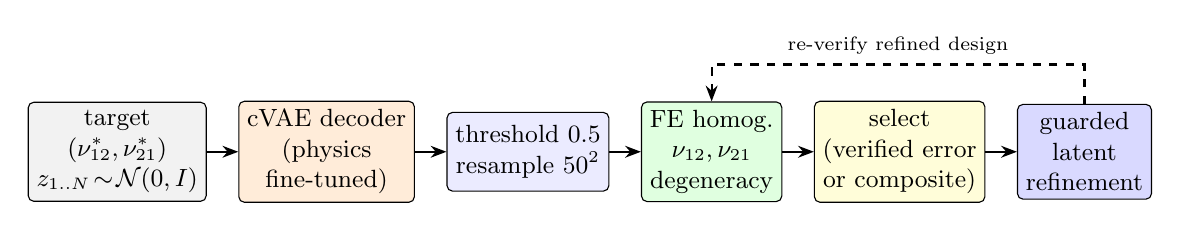
\begin{tikzpicture}[
  node distance=3mm and 4mm,
  box/.style={draw, rounded corners=2pt, align=center, font=\small,
              minimum height=10mm, inner sep=3pt, fill=#1},
  box/.default=white,
  arr/.style={-{Stealth[length=2mm]}, thick}]
\node[box=gray!10] (t) {target\\$(\nu_{12}^{*},\nu_{21}^{*})$\\$z_{1..N}\!\sim\!\mathcal N(0,I)$};
\node[box=orange!15, right=of t] (g) {cVAE decoder\\(physics\\fine-tuned)};
\node[box=blue!8, right=of g] (v) {threshold 0.5\\resample $50^2$};
\node[box=green!12, right=of v] (fe) {FE homog.\\$\nu_{12},\nu_{21}$\\degeneracy};
\node[box=yellow!15, right=of fe] (s) {select\\(verified error\\or composite)};
\node[box=blue!15, right=of s] (r) {guarded\\latent\\refinement};
\draw[arr] (t) -- (g);
\draw[arr] (g) -- (v);
\draw[arr] (v) -- (fe);
\draw[arr] (fe) -- (s);
\draw[arr] (s) -- (r);
\draw[arr, dashed] (r.north) -- ++(0,5mm) -| node[pos=0.25, above, font=\scriptsize]{re-verify refined design} (fe.north);
\end{tikzpicture}
\caption{Inverse-design pipeline. Every candidate is verified by FE
homogenization after the same post-processing that a manufactured design
would undergo. Refinement is detailed in Fig.~\ref{fig:pipeline}.}
\label{fig:framework}
\end{figure}

\subsection{Verified accuracy requires optimizing the verified design}
\label{sec:acc}

\paragraph{Continuous refinement exploits grey densities.}
Refining the continuous decoder output (30 L-BFGS steps, gradients through
the decoder and the exact homogenization sensitivities) helps single samples
of the production model. On set A, $\RR(\nuot)$ rises from 0.874 to 0.976
and the mean absolute error (MAE) of $\nuot$ falls by 57.7\% (95\% CI
49.4--64.6\%; Table~\ref{tab:main}, Fig.~\ref{fig:parity}b). The same
refinement, however, \emph{worsens} the best-of-30 winner: MAE($\nuot$)
rises from 0.0142 to 0.0247, a change of $-73.8\%$ (CI $-119$ to $-39\%$),
and $\RR$ drops from 0.988 to 0.962. The objective trace explains why
(Fig.~\ref{fig:gap}). At the end of continuous refinement the median
objective is $2.5\times10^{-10}$, but the median verified squared error of
the binarized design is $4.4\times10^{-4}$. The optimizer matches the target
on a field whose intermediate densities do not survive thresholding
(Fig.~\ref{fig:refex}). This is the failure mode of surrogate exploitation,
arising inside an exact physics model.

\paragraph{Binarization-aware refinement.}
Placing differentiable counterparts of the verification operators inside the
objective (Fig.~\ref{fig:pipeline}) shrinks the median ratio of verified
error to objective from about $10^{6}$ to about $2\times10^{2}$
(Fig.~\ref{fig:gap}). All pre-specified in-distribution criteria are met
(Table~\ref{tab:main}).
\begin{itemize}
\item \textbf{Single samples.} $\RR(\nuot)$ rises from 0.874 to 0.999 and
MAE($\nuot$) falls by 92.7\% (CI 90.2--94.6\%). The mean relative error of
$\nuot$ drops from 14.4\% to 2.3\%, and $\RR(\nuto)$ rises from 0.477 to
0.875.
\item \textbf{After best-of-30.} MAE($\nuot$) falls by 68.3\% (CI
59.3--75.8\%), $\RR(\nuot)$ rises from 0.988 to 0.998, and MAE($\nuto$)
falls from 0.030 to 0.010 ($\RR(\nuto)$ 0.812 to 0.845). Guarded refinement
accepts 94\% of refinements and gives the same accuracy.
\end{itemize}
Refinement costs 77 FE solves per target on average, i.e.\ about 7\,s of
CPU time on the $50\times50$ grid. Guarding alone does not rescue continuous
refinement after best-of-30 (MAE reduction 10.5\%, CI $-3.0$ to 22.4\%).

\paragraph{Replication on fresh target sets.}
Because the method was developed after continuous refinement had failed on
set A, we repeated it on sets B and C, drawn with different seeds. For single
samples on set B, $\RR(\nuot)$ rises from 0.831 to 0.989 and MAE($\nuot$)
falls by 87.8\% (CI 82.3--92.3\%). After best-of-30, MAE($\nuot$) falls by
59.3\% (CI 46.8--70.9\%) on set B and by 63.6\% (CI 46.3--75.2\%) on set C.
% Sources: p1_6x_in100b_e_a_v2_finetuned.json; p1_9_r5/r6_*_bo30_nofp.json
% (bootstrap computed 2026-10-08 with bootstrap_paired_mae_reduction).

\begin{figure}[t]
\centering
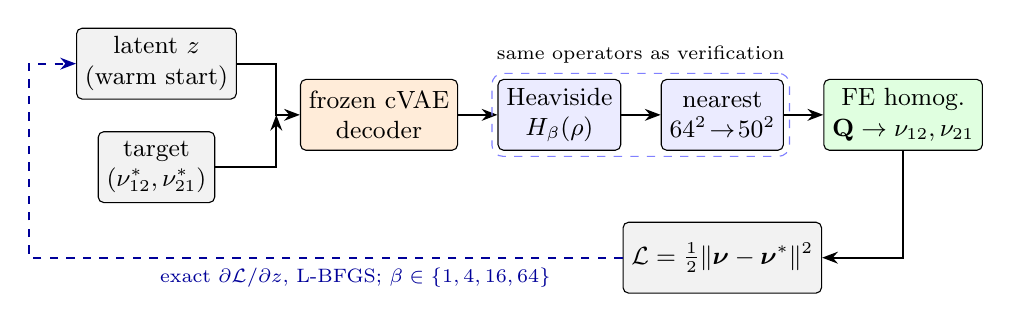
\begin{tikzpicture}[
  node distance=4mm and 5mm,
  box/.style={draw, rounded corners=2pt, align=center, font=\small,
              minimum height=9mm, inner sep=3pt, fill=#1},
  box/.default=white,
  arr/.style={-{Stealth[length=2mm]}, thick},
  grad/.style={-{Stealth[length=2mm]}, thick, dashed, blue!60!black}]
\node[box=gray!10] (z) {latent $z$\\(warm start)};
\node[box=gray!10, below=of z] (c) {target\\$(\nu_{12}^{*},\nu_{21}^{*})$};
\node[box=orange!15, right=8mm of z, yshift=-6.5mm] (dec) {frozen cVAE\\decoder};
\node[box=blue!8, right=of dec] (hv) {Heaviside\\$H_\beta(\rho)$};
\node[box=blue!8, right=of hv] (rs) {nearest\\$64^2\!\to\!50^2$};
\node[box=green!12, right=of rs] (fe) {FE homog.\\$\mathbf{Q}\to\nu_{12},\nu_{21}$};
\node[box=gray!10, below=9mm of rs] (loss) {$\mathcal{L}=\tfrac12\lVert\boldsymbol{\nu}-\boldsymbol{\nu}^{*}\rVert^2$};
\draw[arr] (z) -| ([xshift=-3mm]dec.west) -- (dec.west);
\draw[arr] (c) -| ([xshift=-3mm]dec.west);
\draw[arr] (dec) -- (hv);
\draw[arr] (hv) -- (rs);
\draw[arr] (rs) -- (fe);
\draw[arr] (fe.south) |- (loss.east);
\draw[grad] (loss.west) -- ([xshift=-6mm]loss.west -| z.west)
  node[pos=0.45, below, font=\scriptsize]{exact $\partial\mathcal{L}/\partial z$, L-BFGS; $\beta\in\{1,4,16,64\}$}
  |- (z.west);
\node[draw=blue!50, dashed, rounded corners, fit=(hv)(rs), inner sep=2pt,
      label={[font=\scriptsize]above:same operators as verification}] {};
\end{tikzpicture}
\caption{Binarization-aware latent refinement. The frozen decoder output
passes through differentiable counterparts of the verification operators
before FE homogenization, so the quantity optimized is the quantity verified.
The continuous variant omits the dashed block and uses bilinear resampling.
Verification replaces $H_\beta$ by a hard threshold at 0.5.}
\label{fig:pipeline}
\end{figure}

\begin{table}[t]
\centering
\caption{FE-verified accuracy on set A (100 held-out targets, production
cVAE). $\Delta$MAE is the relative reduction of MAE($\nuot$) versus the
unrefined design of the same mode, with a paired bootstrap 95\% CI. Negative
values mean that refinement made results worse. Joint: mean of
$|\Delta\nuot|+|\Delta\nuto|$. FE: solves per target, including selection.}
\label{tab:main}
\small
\setlength{\tabcolsep}{3.2pt}
\begin{tabular}{llcccccr}
\toprule
Mode & Refinement & $\RR(\nuot)$ & MAE($\nuot$) & $\RR(\nuto)$ & Joint & $\Delta$MAE [95\% CI] & FE\\
\midrule
\multirow{3}{*}{Single}
 & none                 & 0.874 & 0.0517 & 0.477 & 0.127 & -- & 1\\
 & continuous           & 0.976 & 0.0219 & 0.643 & 0.053 & $+57.7\%$ [49.4, 64.6] & 51\\
 & binarization-aware   & \textbf{0.999} & \textbf{0.0038} & \textbf{0.875} & \textbf{0.012} & $\mathbf{+92.7\%}$ [90.2, 94.6] & 78\\
\midrule
\multirow{4}{*}{Best-of-30}
 & none                 & 0.988 & 0.0142 & 0.812 & 0.044 & -- & 30\\
 & continuous           & 0.962 & 0.0247 & 0.671 & 0.052 & $-73.8\%$ [$-119$, $-39$] & 79\\
 & binarization-aware   & \textbf{0.998} & \textbf{0.0045} & 0.845 & 0.014 & $\mathbf{+68.3\%}$ [59.3, 75.8] & 107\\
 & \quad guarded        & \textbf{0.998} & 0.0046 & \textbf{0.846} & 0.014 & $+67.4\%$ [57.9, 75.3] & 107\\
\bottomrule
\end{tabular}
\end{table}

\begin{figure}[t]
\centering
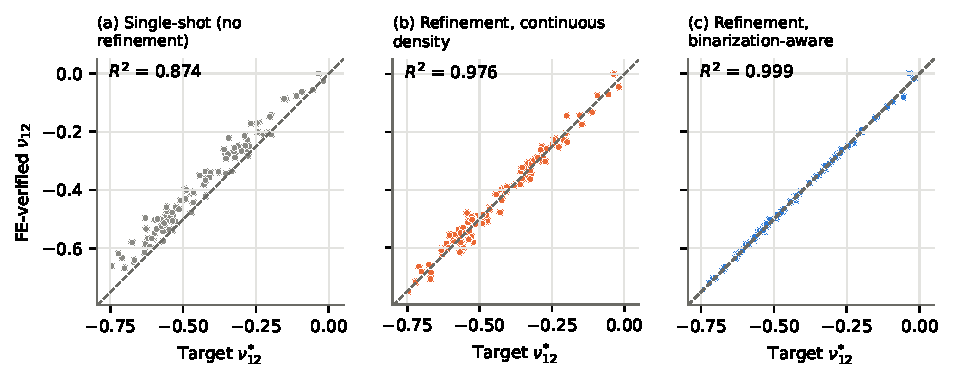
\includegraphics[width=\linewidth]{figures/fig_parity_en.pdf}
\caption{FE-verified versus target $\nuot$ on set A ($n=100$, single samples
of the production cVAE): (a) unrefined; (b) after continuous refinement;
(c) after binarization-aware refinement. All panels start from the same
latent code per condition. Dashed line: identity.}
\label{fig:parity}
\end{figure}

\begin{figure}[t]
\centering
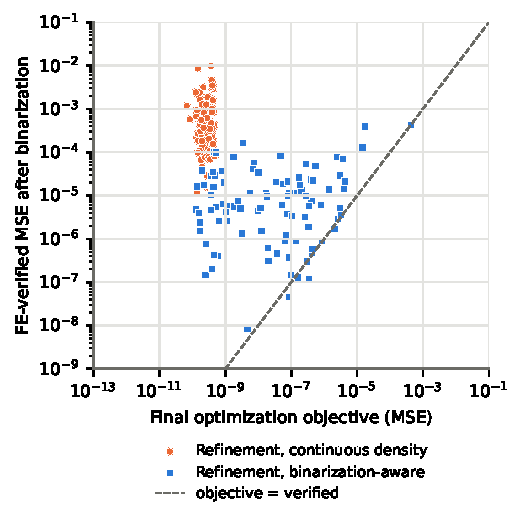
\includegraphics[width=0.55\linewidth]{figures/fig_gap_en.pdf}
\caption{Objective--verification gap. Each point is one condition of set A.
Horizontal axis: final refinement objective; vertical axis: squared
Poisson-ratio error of the binarized design measured by an independent FE
solve. Continuous refinement (circles) reaches objectives near $10^{-10}$
while verified errors remain at $10^{-4}$--$10^{-2}$. Binarization-aware
refinement (squares) moves points towards the identity. Values below
$10^{-14}$ are clipped for display.}
\label{fig:gap}
\end{figure}

\begin{figure}[t]
\centering
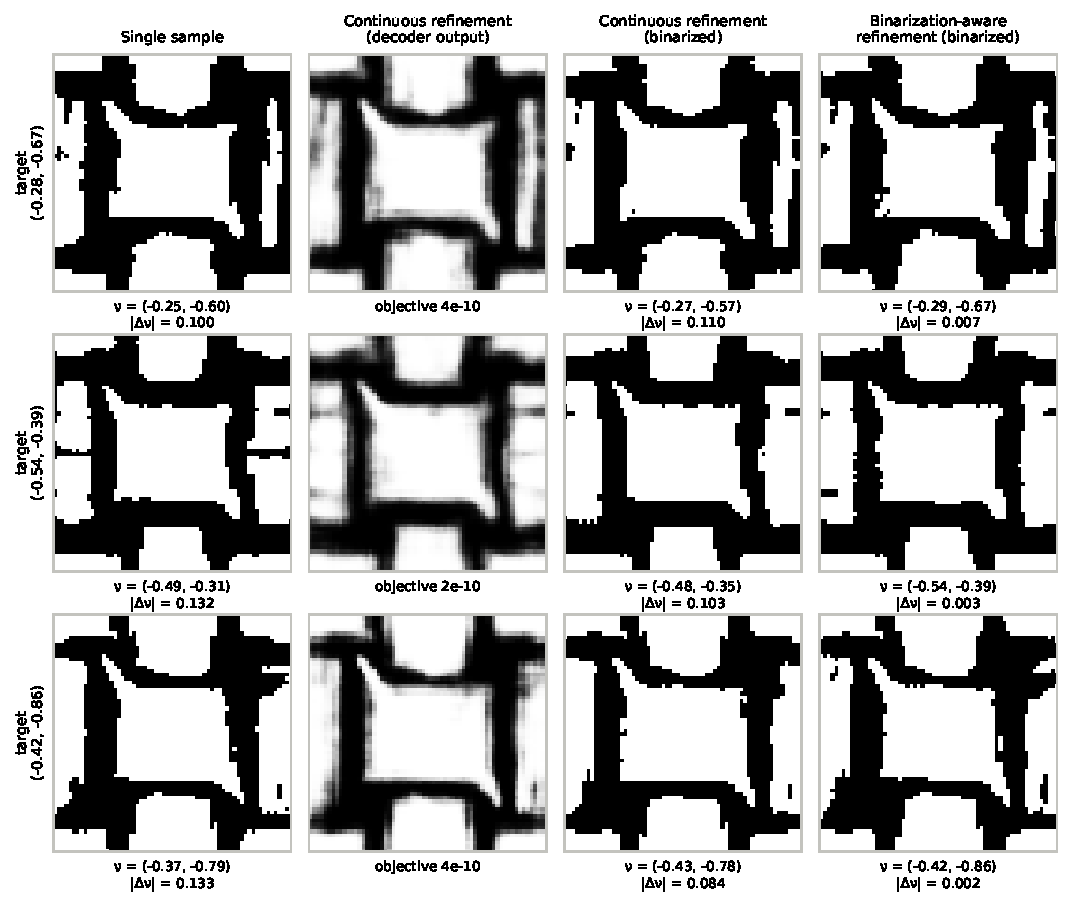
\includegraphics[width=\linewidth]{figures/fig_refine_examples_en.pdf}
\caption{The same starting latent code for three conditions of set A: single
sample, continuous refinement (decoder output and its binarization), and
binarization-aware refinement (binarized). Continuous refinement reaches
its target on a grey field whose binarization has different properties.}
\label{fig:refex}
\end{figure}

\subsection{Comparison with topology optimization from scratch}
\label{sec:simp}

The relevant competitor of a generative pipeline is not a lookup table but
topology optimization run directly for the target. We solved the classical
inverse homogenization problem for every target from four starting
topologies (Section~\ref{sec:to}), verified each result exactly like a
generated design, and kept the best of the four by verified error. This
baseline uses on average 893 FE solves per target (median 102--140\,s of CPU
time on one core), against 107 for best-of-30 sampling followed by guarded
binarization-aware refinement.

\paragraph{Topology optimization shows the same gap.}
At the end of continuation the median error on the projected density field
was $2\times10^{-7}$, whereas the median verified error after thresholding
was $3.6\times10^{-2}$ per run, and for 57\% of the 300 targets the starting
topology with the lowest projected error was not the one with the lowest
verified error. Selection by verified error is therefore necessary for both
methods.

\paragraph{Accuracy, cost and failure mode.}
Table~\ref{tab:simp} compares the two methods on sets A, B and C. On all
three, the generative pipeline matches converged topology optimization in
$\nuot$ ($\RR=0.995$--$0.998$ versus $0.996$--$0.998$) with roughly eightfold
fewer FE solves. Over all targets its joint error is not consistently lower,
because of one failure mode. Every degenerate cell produced by the cVAE (one
in set A, two in set B, none in C) belongs to a target with an anisotropy
ratio $r=\max(\nuto^{*}/\nuot^{*},\,\nuot^{*}/\nuto^{*})\ge10$, which
corresponds to a stiffness ratio $E_2/E_1\ge10$ for an orthotropic cell. In
these cells one column of pixels is empty, so the cell carries no load in one
direction and its Poisson ratio is meaningless (Fig.~\ref{fig:designs}).
For these targets all 30 sampled candidates were disconnected, so the
failure cannot be fixed by selection; only 2.8\% of the training cells have
$r>10$. Without the three degenerate targets, the joint error of the
generative pipeline is 0.0075, 0.0091 and 0.0082 against 0.0127, 0.0140 and
0.0126 for topology optimization, which produced no degenerate cell. The
low $\RR(\nuto)$ of the generative pipeline on sets A and B (0.846, 0.745)
is caused by the same targets.

\paragraph{Stratified, pre-specified confirmation.}
Having observed this on sets A and B, we pre-specified a stratified test on
set C before running it: for targets with $r<10$, the generative pipeline
should have a lower joint error and a lower $\nuot$ error than topology
optimization, with paired 95\% CIs excluding zero. This test was run with the
earlier pipeline that still enforced periodic edges (Appendix~\ref{app:fp}).
The joint-error criterion was met (27\% lower, CI 8--42\%); the $\nuot$
criterion was not (19\% lower, CI $-10$ to 40\%). With the final pipeline,
both criteria are met on all three sets (Table~\ref{tab:simp}); because this
version was not pre-specified, we report it as a sensitivity analysis and
claim parity in $\nuot$ and an advantage in joint error for moderate
anisotropy, not superiority in $\nuot$. Of the five targets with $r\ge10$,
the generative pipeline was better on one (set C) and much worse on four.

\begin{table}[t]
\centering
\caption{Generative pipeline (best-of-30 + guarded binarization-aware
refinement) versus topology optimization from scratch (best of four starts,
converged) on three disjoint sets of 100 held-out targets. Both methods
select by verified joint error. Joint: mean $|\Delta\nuot|+|\Delta\nuto|$.
FE: solves per target. Deg.: degenerate cells ($\min E_i<10^{-3}E_0$).
Manuf.: fraction manufacturable. Bottom rows: relative error reduction of
the generative pipeline versus topology optimization for targets with
anisotropy ratio $r<10$ (paired bootstrap 95\% CI; positive favours the
generative pipeline).}
\label{tab:simp}
\small
\setlength{\tabcolsep}{3.2pt}
\begin{tabular}{llcccccc}
\toprule
Set & Method & $\RR(\nuot)$ & $\RR(\nuto)$ & Joint & FE & Deg. & Manuf.\\
\midrule
\multirow{2}{*}{A} & generative & 0.998 & 0.846 & 0.0139 & 107 & 1 & 0.32\\
 & topology opt. & 0.997 & 0.997 & 0.0128 & 897 & 0 & 0.77\\
\multirow{2}{*}{B} & generative & 0.995 & 0.745 & 0.0229 & 107 & 2 & 0.35\\
 & topology opt. & 0.996 & 0.997 & 0.0139 & 889 & 0 & 0.74\\
\multirow{2}{*}{C} & generative & 0.998 & 0.998 & 0.0082 & 107 & 0 & 0.32\\
 & topology opt. & 0.998 & 0.996 & 0.0126 & 893 & 0 & 0.83\\
\midrule
\multicolumn{8}{l}{$r<10$, joint error: \;A $+41\%$ [26, 54] \;B $+40\%$ [23, 53] \;C $+35\%$ [19, 48]}\\
\multicolumn{8}{l}{$r<10$, $\nuot$ error: \;A $+39\%$ [19, 54] \;B $+39\%$ [19, 54] \;C $+37\%$ [14, 54]}\\
\bottomrule
\end{tabular}
\end{table}

\begin{figure}[t]
\centering
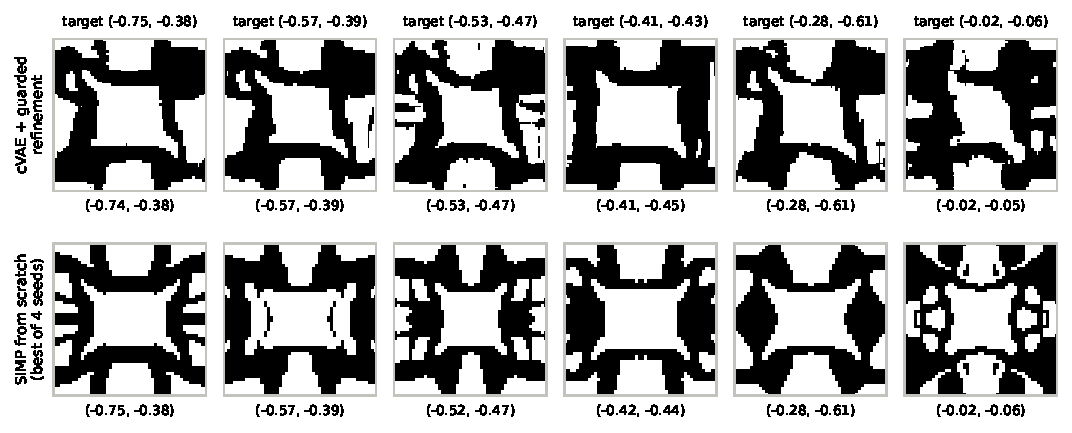
\includegraphics[width=\linewidth]{figures/fig_designs_en.pdf}
\caption{Final designs of the generative pipeline and of topology
optimization from scratch for the same targets of set A, with target and
verified $(\nuot,\nuto)$.}
\label{fig:designs}
\end{figure}

\paragraph{Mesh sensitivity and stiffness.}
All accuracies above are relative to the $50\times50$ FE model used for
data generation, refinement and verification. Re-solving 30 test geometries
with each pixel subdivided into $4\times4$ elements changes $\nuot$ by a
median of 0.015 (3.8\%) and at most 0.042, towards more negative values in
27 of them. The differences in $\nuot$ between the two methods
($\sim\!10^{-3}$) are therefore an order of magnitude smaller than the
discretization error of the model. On the $200\times200$ mesh the ranking of
the two methods on set A is unchanged ($\RR(\nuot)$ 0.992 versus 0.985).
% TODO(P1.10): the 200^2 numbers and fig_stiffness were computed for the
% variant with periodic-edge enforcement (p1_6x_final_design_eval.json).
% Re-run: final_design_eval.py --cvae-json p1_7_c5_in100_bo30_nofp.json
% --out p1_10_final_design_eval_nofp.json (stopped 2026-10-08, battery).
The auxetic designs of both methods are not near-mechanisms: the median
in-plane modulus is $E_1\approx0.07$--$0.08\,E_0$ for both
(Fig.~\ref{fig:stiffness}).

\begin{figure}[t]
\centering
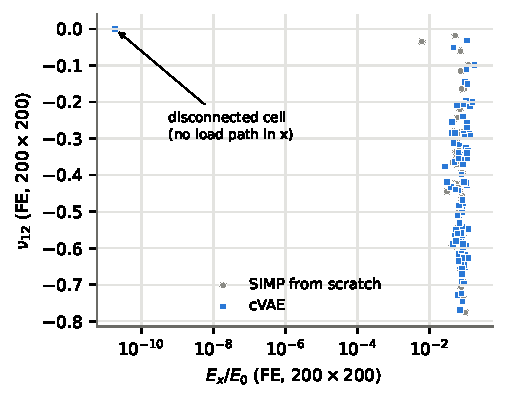
\includegraphics[width=0.6\linewidth]{figures/fig_stiffness_en.pdf}
\caption{Verified $\nuot$ versus $E_1/E_0$ of the final designs on set A,
both on the $200\times200$ mesh. Values computed for the pipeline variant
with periodic-edge enforcement.}
\label{fig:stiffness}
\end{figure}

\paragraph{A hybrid does not inherit the strengths of both.}
Because topology optimization was more robust and more manufacturable while
the generative pipeline was cheaper, we pre-specified a hybrid in which the
generated design initializes topology optimization (continuation
$\beta=8\to64$, at most 61 additional FE solves). It met the cost and
non-degeneracy criteria (166 FE solves per target; 1\% degenerate) but
failed the joint-error non-inferiority criterion against converged
topology optimization (CI lower bound $-96\%$, driven by the one degenerate
target) and the manufacturability criterion (0.33 against a threshold of
0.70). Starting from a sharp projection preserves the topology, including
the thin features, of the generated design. This experiment was run with the
earlier pipeline with periodic-edge enforcement.

\paragraph{Cost.}
The saving of about 790 FE solves per target pays off the $2.7$--$3.0\times10^{6}$
FE solves spent on the training data only after about 3\,500--3\,800
targets (11\,500--12\,700 against the budget-matched variant of topology
optimization). The cost argument therefore holds when many targets must be
served, not for a single design.

\subsection{Retrieval from the training library}
\label{sec:retr}
A lookup in the training library is the cheapest alternative. Verified by
the same chain, the single nearest cell reaches $\RR(\nuot)=0.941$ on set A
and the best of the 30 nearest cells $\RR=0.977$ with a joint error of 0.035,
slightly better than best-of-30 generation without refinement (0.988, joint
error 0.044). Binarization-aware refinement lifts the generative pipeline to
$\RR=0.998$ and a joint error of 0.014. The verified properties of a
training cell also differ from its label: resampling from $64^2$ to $50^2$,
penalization and binarization together shift $\nuot$ by an MAE of 0.032 on
150 test cells, because the labels were computed on the grey SIMP fields.
Labels are thus another quantity that differs from what is verified.
% Source: p1_6x_retrieval_in100_nofp.json; plan.md P1.6y.

\subsection{Manufacturability and multi-objective selection}
\label{sec:multi}

Accurate designs are not automatically buildable. With best-of-30 selection
by verified error and guarded refinement, 32--35\% of the final generated
designs are manufacturable, against 74--83\% for topology optimization
(Table~\ref{tab:simp}). Refinement does not reduce manufacturability: over
four runs (single samples and best-of-30 on set A, best-of-30 on sets B and
C), the manufacturable fraction rose by 4--7 percentage points, with 55
designs becoming manufacturable and 33 ceasing to be (sign test $p=0.025$;
two of the runs share set A).

To trade accuracy against manufacturability during selection, the composite
score of Section~\ref{sec:verify} can replace the verified error. On 300 test
targets ($N=30$), composite selection keeps $\RR(\nuot)=0.988$ (0.997 with
accuracy-only selection) while every first sample is auxetic; 23.8\% of all
generated samples are manufacturable (Table~\ref{tab:multi}). This $\RR$
differs from that of Table~\ref{tab:main} because the targets and the latent
draws differ. To test whether the scalarization respects the multi-objective
structure, we computed, for 24 targets with 30 candidates each, the
Spearman correlation between the composite score and the non-dominated
sorting rank over the three raw objectives (Fig.~\ref{fig:spearman}). All 24
correlations were positive (0.45--0.86, median 0.746, mean 0.718). The
pre-specified criterion (mean $\ge0.7$) was set for, and failed with, the
earlier pipeline (mean 0.693); we therefore read the composite score as
agreeing moderately, not strongly, with the Pareto structure. That the
selected candidate lies on the first Pareto front is guaranteed for positive
weights and is not evidence.

Figure~\ref{fig:tiling} shows that the generated cells tile without edge
matching, and Fig.~\ref{fig:deformation} shows the deformation mechanism of a
generated auxetic cell and of a generated cell with $\nuot>0$.

\begin{table}[t]
\centering
\caption{Selection on 300 test targets (best-of-30, no refinement). Hit
rate: fraction of targets whose first sample is auxetic ($\nuot<0$).
Manufacturable: share of all generated samples.}
\label{tab:multi}
\small
\begin{tabular}{lccc}
\toprule
Selection & $\RR(\nuot)$ & Hit rate, first sample & Manufacturable samples\\
\midrule
Verified accuracy only  & 0.997 & 1.00 & 0.238\\
Composite score         & 0.988 & 1.00 & 0.238\\
\midrule
\multicolumn{4}{p{0.85\linewidth}}{Composite score vs.\ Pareto rank (24 targets $\times$ 30 candidates): Spearman mean 0.718, median 0.746, range 0.45--0.86; 24/24 positive.}\\
\bottomrule
\end{tabular}
\end{table}

\begin{figure}[t]
\centering
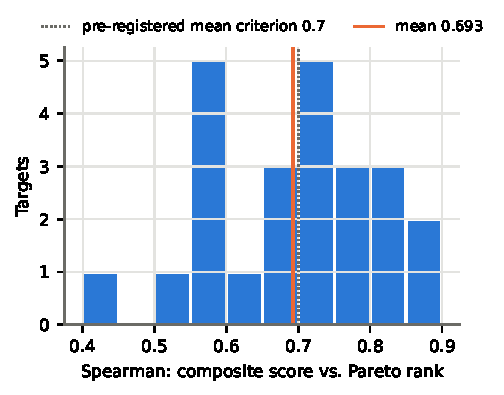
\includegraphics[width=0.5\linewidth]{figures/fig_spearman_en.pdf}
\caption{Distribution over 24 targets of the Spearman correlation between the
composite score and the Pareto rank of 30 candidates (objectives: verified
$|\Delta\nuot|$, manufacturability score, aesthetic score). Dotted:
pre-specified threshold for the mean.}
\label{fig:spearman}
\end{figure}

\begin{figure}[t]
\centering
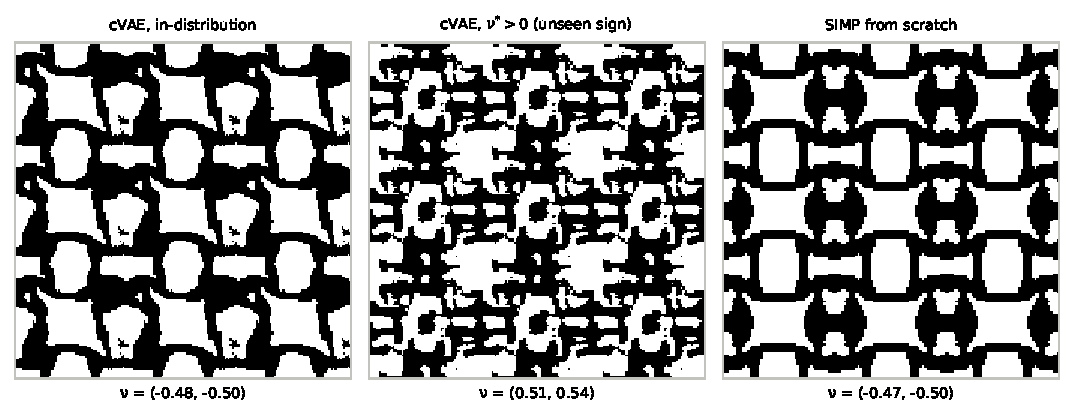
\includegraphics[width=0.85\linewidth]{figures/fig_tiling_en.pdf}
\caption{$3\times3$ tilings of final designs: generative pipeline in
distribution, generative pipeline for an unseen sign ($\nuot^{*}>0$), and
topology optimization from scratch. Periodic boundary conditions on the
element mesh make every pixel cell tile by translation.}
\label{fig:tiling}
\end{figure}

\begin{figure}[t]
\centering
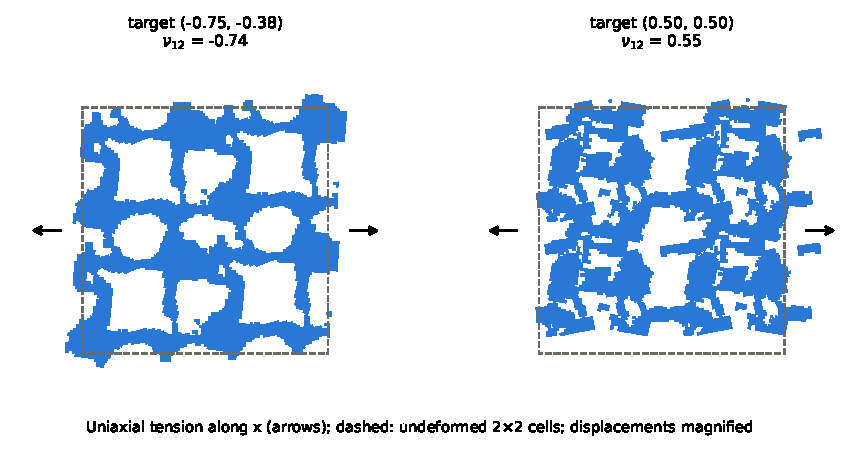
\includegraphics[width=0.85\linewidth]{figures/fig_deformation_en.pdf}
\caption{Deformation under uniaxial tension along $x$ (FE, $50\times50$,
displacements magnified) of a generated auxetic cell (target
$(\nuot^{*},\nuto^{*})=(-0.75,-0.38)$, verified $\nuot=-0.744$) and of a
generated cell for $\nuot^{*}=\nuto^{*}=0.5$ (verified 0.547). Dashed: the
undeformed $2\times2$ cells.}
\label{fig:deformation}
\end{figure}

\subsection{Out-of-distribution targets}

\paragraph{Admissible targets.}
For a two-dimensional orthotropic material, positive definiteness of the
compliance requires $\nuot\nuto<1$ \citep{lempriere1968poisson}. Symmetric
targets $\nuot^{*}=\nuto^{*}\le-1$ are therefore infeasible. In the training
data the most negative $\nuot=-1.95$ is paired with $\nuto=-0.04$, and the
largest product $\nuot\nuto$ is 0.43. An earlier ``extreme auxetic'' test in
our project used targets such as $(-2.1,-2.1)$, all of which violate the
bound; we exclude such targets. Out-of-range magnitude targets below are
anisotropic, with $\nuto^{*}=-0.05$.

\paragraph{Sign: the generator reaches unseen signs, but topology
optimization is more accurate.}
Every training cell is auxetic ($-1.95\le\nuot\le-0.002$), so retrieval
cannot return $\nuot>0$; for the 28 sign-flip targets its error is at least
0.33--0.37 on average. Best-of-30 generation followed by guarded
binarization-aware refinement produced the correct sign for most targets
and reduced the MAE of $\nuot$ by 66--73\% relative to best-of-30 alone
(Table~\ref{tab:signflip}, Fig.~\ref{fig:signflip}). Topology optimization
from scratch, however, was markedly more accurate in all three groups, also
when only targets with non-degenerate designs from both methods are
compared. Both methods produced degenerate designs (three each). The three
degenerate cells from topology optimization are empty: with all elements at
$E_{\min}$, the cell has the Poisson ratio of the base material, 0.3, and an
unguarded verifier scores it as a near-perfect answer to targets between 0.25
and 0.30. Only 8--12\% of the generated cells for these targets were
manufacturable, against 75\% for topology optimization.

\begin{table}[t]
\centering
\caption{Sign-flip targets ($\nuot^{*}>0$; training data contain only
$\nuot<0$). MAE of FE-verified $\nuot$: retrieval (lower bound, since every
training label is $\le-0.002$), generative pipeline before and after
guarded refinement, and topology optimization (TO). In brackets: MAE over
targets for which neither method returned a degenerate design ($n$ in the
last column). Deg.: degenerate designs, generative / TO.}
\label{tab:signflip}
\small
\setlength{\tabcolsep}{3.5pt}
\begin{tabular}{lcccccc}
\toprule
Group & Retrieval & Best-of-30 & + refinement & TO & Deg. & $n$\\
\midrule
$\nuot^{*}=\nuto^{*}$ (12)  & $\ge0.33$ & 0.204 & 0.056 [0.030] & 0.012 [0.009] & 1 / 2 & 9\\
$\nuto^{*}=0.1$ (8)          & $\ge0.37$ & 0.272 & 0.090 [0.054] & 0.031 [0.032] & 1 / 0 & 7\\
$\nuto^{*}=0.3$ (8)          & $\ge0.37$ & 0.222 & 0.076 [0.033] & 0.005 [0.006] & 1 / 1 & 6\\
\midrule
FE per target & -- & 30 & 105--107 & 761--826 & & \\
\bottomrule
\end{tabular}
% Sources: p1_9_r7_signflip_*_nofp.json, p1_6b_simp_*.json,
% p1_10_degenerate_check.json (2026-10-08).
\end{table}

\begin{figure}[t]
\centering
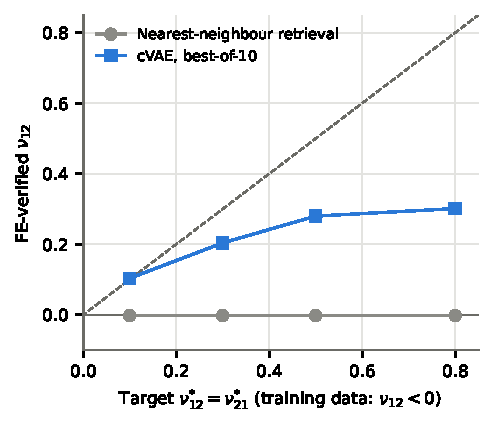
\includegraphics[width=0.5\linewidth]{figures/fig_signflip_en.pdf}
\caption{Symmetric sign-flip targets: FE-verified $\nuot$ of the generative
pipeline (best-of-30 and after guarded refinement) and of topology
optimization from scratch. Retrieval is bounded by the training library
($\nuot\le-0.002$, grey line). Open markers: degenerate designs. Dashed:
identity.}
\label{fig:signflip}
\end{figure}

\paragraph{Magnitude: refinement extends into sparse data but not beyond.}
We swept $\nuot^{*}\in\{-1.0,$ $-1.5,$ $-1.75,$ $-2.0,$ $-2.25,$ $-2.5\}$
($\nuto^{*}=-0.05$) with ten independent latent draws per target and
best-of-30 selection (Table~\ref{tab:ood}, Fig.~\ref{fig:ood}). The training
data thin out well before their minimum: 88 training samples have
$\nuot<-1.5$, 14 have $\nuot<-1.75$ and two have $\nuot<-1.9$, all of them
$90^{\circ}$ rotations of cells with extreme $\nuto$. Binarization-aware
refinement reaches a median relative error of 0.3\% at $-1.75$ and 1.2\% at
$-2.0$, which meets the pre-specified 8\% criterion at $-2.0$. The
distribution there is bimodal, however: six of the ten repeats end below
1.7\%, four between 17\% and 31\%. From $-2.25$ onwards every variant
saturates, and unguarded refinement is worse than no refinement. Refinement
is a local search in the latent space of the decoder and cannot create
magnitudes the decoder never learned to represent.

\begin{table}[t]
\centering
\caption{Anisotropic magnitude sweep ($\nuto^{*}=-0.05$; best-of-30;
10 repeats per target). Entries: median relative error of FE-verified
$\nuot$. The training range of $\nuot$ ends at $-1.95$.}
\label{tab:ood}
\small
\begin{tabular}{lcccccc}
\toprule
$\nuot^{*}$ & $-1.0$ & $-1.5$ & $-1.75$ & $-2.0$ & $-2.25$ & $-2.5$\\
\midrule
Best-of-30, no refinement        & 0.5\% & 0.8\% & 3.6\% & 10.1\% & 15.6\% & 21.7\%\\
+ continuous refinement          & 1.3\% & 1.2\% & 3.5\% & 31.0\% & 41.6\% & 45.5\%\\
+ binarization-aware refinement  & 0.4\% & 0.2\% & 0.3\% & \textbf{1.2\%} & 24.7\% & 28.8\%\\
+ binarization-aware, guarded    & 0.1\% & 0.2\% & 0.3\% & \textbf{1.2\%} & 14.2\% & 20.0\%\\
\bottomrule
\end{tabular}
\end{table}

\begin{figure}[t]
\centering
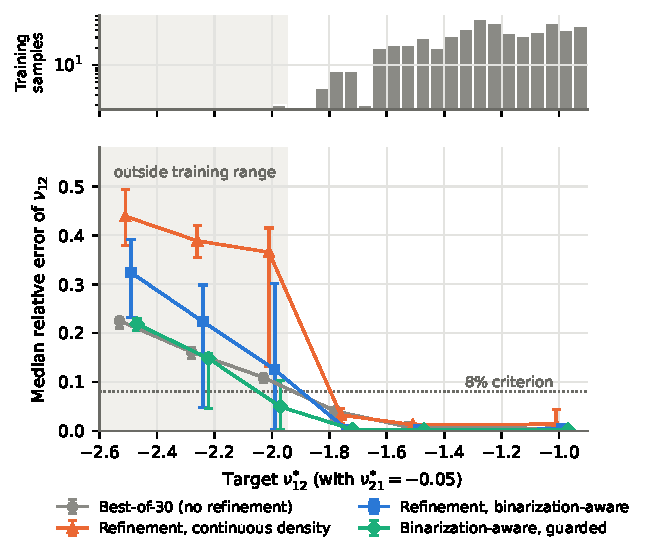
\includegraphics[width=0.62\linewidth]{figures/fig_ood_en.pdf}
\caption{Top: number of training samples per bin of $\nuot$ (log scale).
Bottom: median relative error of FE-verified $\nuot$ versus target
($\nuto^{*}=-0.05$). Error bars: interquartile range over 10 latent draws per
target; markers offset horizontally for legibility. Shaded: outside the
training range. Dotted: pre-specified 8\% criterion at $\nuot^{*}=-2.0$.}
\label{fig:ood}
\end{figure}

\subsection{Architecture ablations}

\paragraph{KAN versus linear heads.}
We replaced the three linear layers of the cVAE (latent mean, log-variance
and decoder bottleneck) with Kolmogorov--Arnold layers \citep{liu2024kan}.
Both heads were trained with identical recipes, hyperparameters and seeds
(123 and 7). KAN was declared the winner only if the paired CI excluded zero
for both seeds. It did not win in any mode (Table~\ref{tab:kan}). In the
production mode (best-of-30 without refinement), the linear head was
significantly better for both seeds. With refinement, both heads reached
$\RR(\nuot)=0.997$--$0.999$. The KAN head has $3.2\times$ more parameters
(4.79\,M versus 1.49\,M) and needs about $1.6\times$ the time per epoch, so
we retain the linear head. This ablation was evaluated with the earlier
pipeline with periodic-edge enforcement, which does not change accuracy on
set A (Appendix~\ref{app:fp}).

\begin{table}[t]
\centering
\caption{Controlled KAN versus linear ablation on set A (two seeds).
$\Delta$MAE: relative reduction of MAE($\nuot$) of KAN versus linear
(positive favours KAN), paired bootstrap 95\% CI. Bold: CI excludes zero.}
\label{tab:kan}
\small
\setlength{\tabcolsep}{4pt}
\begin{tabular}{lcccc}
\toprule
 & \multicolumn{2}{c}{$\RR(\nuot)$ Linear / KAN} & \multicolumn{2}{c}{$\Delta$MAE KAN vs.\ Linear}\\
\cmidrule(lr){2-3}\cmidrule(lr){4-5}
Mode & seed 123 & seed 7 & seed 123 & seed 7\\
\midrule
Single sample              & 0.852 / 0.904 & 0.815 / 0.911 & $+13.3\%$ [$-0.2$, 24.4] & $\mathbf{+18.2\%}$ [3.8, 30.4]\\
Single sample + refinement & 0.994 / 0.997 & 0.998 / 0.999 & $+33.2\%$ [$-15.1$, 60.5] & $\mathbf{+33.9\%}$ [11.7, 52.3]\\
Best-of-30                 & 0.977 / 0.974 & 0.982 / 0.980 & $\mathbf{-25.2\%}$ [$-56.2$, $-1.0$] & $\mathbf{-19.9\%}$ [$-42.1$, $-1.7$]\\
Best-of-30 + refinement    & 0.998 / 0.997 & 0.998 / 0.999 & $+11.3\%$ [$-38.7$, 43.6] & $\mathbf{+44.1\%}$ [24.9, 59.7]\\
\bottomrule
\end{tabular}
\end{table}

\paragraph{Implicit wavelet decoder.}
A resolution-agnostic WIRE decoder \citep{saragadam2023wire} was given one
final attempt. It combined Heaviside projection inside the physics loss, no
forced symmetry and the two-stage recipe. The pre-specified criteria were a
single-sample hit rate of at least 30\% and a positive FE $\RR$ on 24
held-out targets. It reached a hit rate of 12.5\% and an FE $\RR$ of $-7.19$
after best-of-30, against a hit rate of 100\% for the convolutional decoder,
and only 4.6\% of its samples were manufacturable. We therefore closed this
direction.

% ---------------------------------------------------------------------------
\section{Discussion}

\paragraph{Optimizing what is verified.}
The central finding is that any gradient-based search over density fields,
whether in the latent space of a generative model or over element densities
in topology optimization, will exploit the difference between the field it
differentiates and the binarized design that is finally analysed. The
optimizer reaches objectives of $10^{-10}$ on fields that the verifier sees
very differently (Fig.~\ref{fig:gap}), and the same happens in topology
optimization with Heaviside continuation to $\beta=64$. The gap is invisible
in the loss curve. Three remedies follow, and all are cheap: include the
verification operators in the objective, select among candidates by verified
rather than optimized error, and treat degenerate cells as failures in the
verifier itself. Neither of the first two ingredients is new in
density-based topology optimization \citep{guest2004achieving,wang2011projection};
what this work shows is that omitting them changes the conclusions of a
comparison between methods, and that the generative and the classical route
need them equally. The third is easy to overlook: an empty cell has the
Poisson ratio of its base material, and in our sign-flip test such cells
were the best answers that topology optimization returned for three targets.

\paragraph{What a generative model adds.}
Measured against converged topology optimization rather than against a
lookup table, the advantage of the generative pipeline is narrower than is
commonly implied, in line with the critical review of
\citet{woldseth2022use}. It reaches the same verified accuracy with about
eight times fewer FE solves per target, and a lower joint error for targets
of moderate anisotropy, but the saving is amortized only after thousands of
targets because the training data themselves were produced by topology
optimization. Without refinement, retrieval from the same library is about
as accurate. The pipeline is therefore attractive when many targets must be
served, for example in interactive design or in the inner loop of a
multiscale optimization, and not when a single cell is needed. Its failures
are predictable: strongly anisotropic targets that are sparse in the
training data. Reporting such failures by stratum, rather than averaging
them into a single score, made them visible in our study.

\paragraph{Manufacturability and out-of-distribution targets.}
Topology optimization from scratch produced connected cells with adequate
feature size more than twice as often as the generative pipeline. Latent
refinement slightly increased that fraction, and initializing topology
optimization with the generated design did not recover it, because a sharp
initial projection preserves the generated topology. For non-auxetic targets
the cVAE reaches the correct sign where retrieval from the library cannot,
but topology optimization reaches the target far more accurately. Along
magnitude, refinement pushes into regions with only a handful of training
samples, but all generative variants stop where the data end. OOD claims
for generative models should therefore name the direction in property space,
check that the target is physically admissible, and compare against
topology optimization rather than retrieval. Magnitude extrapolation will
likely require new training data near the boundary.

\paragraph{Limitations.}
(i) Accuracy is measured against a $50\times50$ linear-elastic,
small-strain FE model with $\nu_0=0.3$; its discretization error (median
0.015 in $\nuot$) exceeds the reported mean errors. Large strain, other base
materials and three-dimensional cells are not addressed, and no design was
tested experimentally.
(ii) The generative pipeline fails for strongly anisotropic targets
($r\ge10$), which are sparse in the training data; topology optimization does
not.
(iii) Topology optimization produces manufacturable cells more than twice as
often (0.74--0.83 versus 0.32--0.35).
(iv) For targets with an unseen sign, topology optimization is markedly more
accurate; the advantage of the generative model in that regime holds only
against retrieval.
(v) The cost advantage is amortized over about 3\,500 targets.
(vi) The aesthetic score is a heuristic that has not been validated against
human judgement.
(vii) The method of refinement was chosen after a failure on set A; the
replication on sets B and C and the pre-specified test on set C mitigate,
but do not remove, this dependence.

\section{Conclusions}
Refining generated metamaterial cells with exact physics is only reliable if
the objective is evaluated on the design that will be verified: binarized,
resampled and checked for degeneracy. With this change, a cVAE with
latent refinement matches converged topology optimization in $\nuot$ with
about eight times fewer FE solves and achieves a lower joint error for
moderately anisotropic targets, replicated on three disjoint target sets.
Topology optimization from scratch remains the better choice for strongly
anisotropic targets, for manufacturability and for targets outside the
training data. The same principle applies to topology optimization itself:
the verified design, not the projected field, is what has to be optimized
and compared.

\appendix
\section{Periodic-edge enforcement}
\label{app:fp}
The earlier pipeline replaced opposite boundary columns and rows by their
mean before thresholding, both at verification and inside refinement, and
counted edge mismatch in the manufacturability score. Because the FE mesh
uses periodic boundary conditions on elements, every pixel cell tiles by
translation and this step is unnecessary. It also moved the verified
properties of training cells away from their labels (MAE in $\nuot$ 0.055
with the step, 0.032 without). On set A, removing it left the accuracy after
best-of-30 and refinement unchanged. The decision to remove it was made
before the numbers of this paper were recomputed; several results improved
afterwards, which is why both versions are reported. Main changes (with
$\to$ without): single-sample refinement $\Delta$MAE $+91.8\%\to+92.7\%$;
best-of-30 refinement $\Delta$MAE $+62.6\%\to+68.3\%$; manufacturable after
best-of-30 and guarded refinement $0.24\to0.32$ (with the edge criterion
removed from the definition); magnitude sweep at $\nuot^{*}=-2.0$, aware
refinement, $12.5\%\to1.2\%$; joint-error advantage at $r<10$ on set C
$+27\%\to+35\%$, $\nuot$ advantage $+19\%$ (CI includes zero) $\to+37\%$;
Spearman mean of the composite score $0.693\to0.718$. The pre-specified
results (set C stratified test, hybrid) are those obtained with the step.
% Source: plan.md "Kết quả P1.9"; p1_7_c5_comparison.json.

% ---------------------------------------------------------------------------
\section*{Statements and declarations}

\paragraph{Replication of results.}
Code (data generation, FE homogenization with exact sensitivities, cVAE
training, refinement, topology-optimization baseline), trained checkpoints,
the target sets and all per-target outputs underlying the tables and figures
will be made available at [repository URL and Zenodo DOI to be inserted].
Every number in the paper is produced by scripts in
\texttt{docs/paper1/scripts} from these outputs.

\paragraph{Funding.} [To be completed.]

\paragraph{Competing interests.} The author declares no competing
interests. [To be confirmed.]

\paragraph{Use of generative AI.} [To be completed by the author: AI
assistance (Claude, Anthropic) was used for code development, data analysis
and drafting of the manuscript; the author reviewed all content and takes
full responsibility for it.]

\paragraph{Author contributions.} [CRediT statement to be completed.]

\bibliographystyle{unsrtnat}
\bibliography{refs}

\end{document}
